\documentclass[10pt]{beamer}
\usepackage[utf8]{inputenc}
\usepackage[T1]{fontenc}
\usepackage{babel}
\usepackage{tikz}
\usepackage{quantikz}
\usepackage{amsmath}
\usepackage{physics}
\usepackage{graphicx}
% \usepackage{tikz-cd}
%\pgfdeclarelayer{nodelayer}
%\pgfdeclarelayer{edgelayer}
%\pgfsetlayers{nodelayer,edgelayer}

%\tikzcdset{every matrix/.style={ampersand replacement=\&}}

\usetheme{metropolis}

\definecolor{zx_red}{RGB}{232, 165, 165}
\definecolor{zx_green}{RGB}{216, 248, 216}
\definecolor{had_yellow}{RGB}{221, 218, 28}

\tikzstyle{gn}=[circle,rounded corners=0.8em,fill=zx_green,draw=black,
  line width=0.8 pt,inner sep=3pt,minimum width=1.5em,minimum height=1.5em]
\tikzstyle{rn}=[circle,rounded corners=0.8em,fill=zx_red,draw=black,
  line width=0.8 pt,inner sep=3pt,minimum width=1.5em,minimum height=1.5em]
\tikzstyle{had}=[rectangle,fill=had_yellow,draw=black,
  line width=0.8 pt,inner sep=3pt,minimum width=1.5em,minimum height=1.5em]

\usepackage{appendixnumberbeamer}

\usepackage{booktabs}
\usepackage[scale=2]{ccicons}

\usepackage{pgfplots}
\usepgfplotslibrary{dateplot}

\usepackage{xspace}
\newcommand{\themename}{\textbf{\textsc{metropolis}}\xspace}

\title{ZX-račun}
\subtitle{Nov pristop h kvantnem računalništvu}
\date{\today}
\author{Tadej Petrič}
\institute{Fakulteta za matematiko in fiziko}
% prednosti kvantnega računalništva vs klasično
% kvantna mehanika
% klasično kvantno rač
% 4+ zx
\begin{document}
\begin{frame}
  \maketitle
\end{frame}
\begin{frame}
  \frametitle{Kvantno računalništvo}
  \begin{itemize}
  \item Klasično počasne probleme želimo rešiti hitreje
  \item Lastnosti kvantne mehanike omogočijo nove pristope
  \item Faktorizacija števil (verjetno) počasna
  \item Iskanje inverza funkcije počasno
  \pause\item Shorov algoritem, Groverjev algoritem
  \end{itemize}
\end{frame}
\begin{frame}
  \frametitle{Osnove klasičnega računalništva}
  \begin{itemize}
  \item Prisotna električna napetost ali pa ne
  \item Klasične vrednosti \(1\) in \(0\) (biti)
    \begin{itemize}
    \item Označimo \(\ket1\) in \(\ket0\), da razločimo od števil
    \end{itemize}
  \item Logična vrata \(\land\), \(\lor\), \(\lnot\)
  \item Bite lahko brišemo \(\ket0\land x \mapsto \ket0\)
  \item Bite lahko kopiramo (razcep žic)
  \item Stanje računalnika opišemo s skupino zaporednih bitov
    \begin{itemize}
    \item Primer \(\ket{00101} = (0,0,1,0,1)\)
    \item Na skupinah lahko uporabljamo logična vrata
    \end{itemize}
  \end{itemize}
\end{frame}
\begin{frame}
  \frametitle{Kubiti}
  \begin{itemize}
  \item Kubiti so kvantna verzija bitov
  \item Lahko mešanica \(\ket0\) in \(\ket1\)
  \item Predstavimo kot linearno kombinacijo \(a\ket0 + b\ket1\)
  \item Zahtevamo \(a^2+b^2 = 1\) kot robni pogoj
  \item Fizikalno ponavadi predstavimo s spinom delcov (navidezno vrtenje okoli (X,Y,Z) osi)
  \item Ko jih izmerimo, dobimo klasično vrednost \(\ket0\) ali \(\ket1\)\pause
    \begin{itemize}
    \item Vrednosti meritve ne vemo vnaprej
    \item Vemo le verjetnost, da izmerimo določeno vrednost
    \item Za meritvijo vrednost ostane ista
    \end{itemize}
  \end{itemize}
\end{frame}
\begin{frame}
  \frametitle{Skupine kubitov}
  \begin{itemize}
  \item Pomembni so sistemi večih kubitov
  \item Kubiti so med seboj lahko prepleteni
    \begin{itemize}
    \item Ko dobimo informacijo o kubitu, dobimo informacijo o kubitih, s katerimi je prepleten
    \end{itemize}\pause
  \item Primer \(\frac1{\sqrt2}(\ket{00}+\ket{11})\)
    \begin{itemize}
    \item Dva prepletena kubita\pause
    \item Na prvem izmerimo \(\ket0\) ali \(\ket1\) z enako verjetnostjo
    \item Če za tem izmerimo drugi kubit, bo z verjetnostjo \(1\) odgovor enak kot pri prvem
    \end{itemize}
  \end{itemize}
\end{frame}
\begin{frame}
  \frametitle{Kloniranje in brisanje}
  Lastnosti kvantnih vrat
  \begin{itemize}
  \item Kubitov ne moremo klonirati
    \begin{itemize}
    \item Ne obstajajo vrata \(\forall x.\, \ket{0x}\mapsto\ket{xx}\)
    \item Vrata bodo imela kvečjemu manj izhodov kot vhodov
    \end{itemize}\pause
  \item Kubitov ne moremo brisati
    \begin{itemize}
    \item Ekvivalentno prejšnji trditvi, če čas teče v preteklost
    \item Ne obstajajo vrata \(\forall x.\, \ket x\mapsto\ket0\)
    \item Vrata kvečjemu več izhodov kot vhodov
    \end{itemize}\pause
  \item Vrata enako število vhodov kot izhodov
  \item Če te trditvi ne bi držali, bi lahko komunicirali hitreje od svetlobe!
  \end{itemize}
\end{frame}
\begin{frame}[fragile]
  \frametitle{Kvantna vezja}
  \begin{itemize}
  \item Kubite lahko predstavimo z vektorji dolžine \(1\) v bazi \(\ket0, \ket1\)
  \item Kvantna vrata predstavimo z unitarnimi preslikavami
  \end{itemize}
  Vezja lahko narišemo tudi z diagramom:\\
  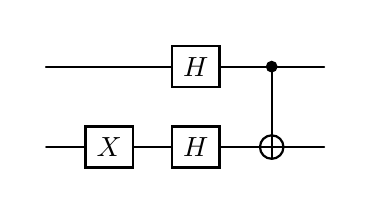
\begin{tikzpicture}
    \node[scale=1.0] {
      \begin{quantikz}
        \qw & \qw       & \gate{H} & \ctrl{1} & \qw \\
        \qw & \gate{X}  & \gate{H} & \targ{}  & \qw
      \end{quantikz}
    };
  \end{tikzpicture}\\
  Tukaj 3 unarna vrata (X, H) in ena binarna (C-NOT)
\end{frame}
\begin{frame}
  \frametitle{Težave}
  \pause
  \begin{itemize}
  \item Za večja vezja zelo nepregledna \pause
  \item Če dve vezji predstavljata isto transformacijo, ne poznamo (vedno) pravil, ki bi prvo pretvorila v drugo\pause
  \item Veliko trditev o kvantni mehaniki težko dokazati
  \end{itemize}
\end{frame}






\begin{frame}
  \frametitle{ZX-Račun}
  Vezje predstavimo kot graf. Definiramo dva tipa vozlišč: X pajek (rdeč) in Z pajek (zelen)\\
  Lahko imata poljubno število vhodov ali izhodov\\
  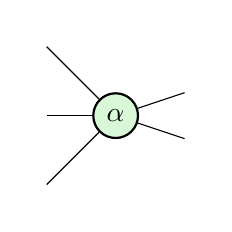
\begin{tikzpicture}
    %\begin{pgfonlayer}{nodelayer}
    \node (01) at (0, 0) {};
    \node (02) at (0, 1) {};
    \node (03) at (0, 2) {};
    \node [style=gn] (1) at (1.00, 1.00) {\(\alpha\)};
    \node (21) at (2, 0.66666) {};
    \node (22) at (2, 1.33333) {};
    %\end{pgfonlayer}
    %\begin{pgfonlayer}{edgelayer}
    \draw (01) to (1);
    \draw (02) to (1);
    \draw (03) to (1);
    \draw (1) to (21);
    \draw (1) to (22);
    %\end{pgfonlayer}
  \end{tikzpicture}\\
  Ta pajek ustreza preslikavi
  \begin{align*}
    \ket{00}\bra{000} + e^{i\alpha}\ket{11}\bra{111}
  \end{align*}
  Neformalno \(\bra{000}\) predstavlja kolikšen del vhodnega kubajta je \(\ket{000}\)
\end{frame}
\begin{frame}
  \frametitle{Več o pajkih}
  Rdeč pajek (X) se obnaša podobno kot Z pajek, le da v bazi \(\{\ket{-},\ket{+}\}\) namesto \(\{\ket0,\ket1\}\)\\
  Kadar je \(\alpha = 0\), oznake ne pišemo
  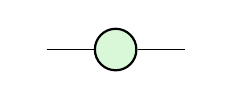
\begin{tikzpicture}
    \node (0) at (0,0) {};
    \node [style=gn] (1) at (1,0) {};
    \node (2) at (2,0) {};
    \draw (0) to (1);
    \draw (1) to (2);
  \end{tikzpicture}\\
  Očitno ne predstavljajo več unitarnih preslikav
\end{frame}
\begin{frame}
  \frametitle{Hadamardova vrata}
  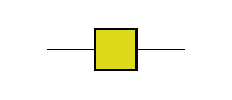
\begin{tikzpicture}
    \node (0) at (0,0) {};
    \node [style=had] (1) at (1,0) {};
    \node (2) at (2,0) {};
    \draw (0) to (1);
    \draw (1) to (2);
  \end{tikzpicture}\\
  Hadamardova vrata spreminjajo bazo. Lahko definiramo kot kompozicijo Z in X pajkov\\
  \vspace{3mm}
  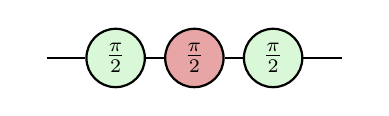
\begin{tikzpicture}
    \node (0) at (0.00, 0.00) {};
    \node [style=gn] (1) at (1, 0) {\(\frac\pi2\)};
    \node [style=rn] (2) at (2, 0) {\(\frac\pi2\)};
    \node [style=gn] (3) at (3, 0) {\(\frac\pi2\)};
    \node (4) at (4.00, 0.00) {};
    \draw (0) to (1);
    \draw (1) to (2);
    \draw (2) to (3);
    \draw (3) to (4);
  \end{tikzpicture}\\\pause{}
  Če imamo\vspace{3mm}\\
  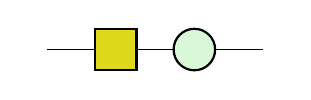
\begin{tikzpicture}
    \node (0) at (0,0) {};
    \node [style=had] (1) at (1,0) {};
    \node [style=gn] (2) at (2,0) {};
    \node (3) at (3,0) {};
    \draw (0) to (1);
    \draw (1) to (2);
    \draw (2) to (3);
  \end{tikzpicture}\\
  Lahko to pretvorimo v\vspace{3mm}\\
  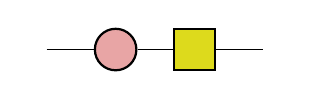
\begin{tikzpicture}
  \node (0) at (0,0) {};
  \node [style=rn] (1) at (1,0) {};
  \node [style=had] (2) at (2,0) {};
  \node (3) at (3,0) {};
  \draw (0) to (1);
  \draw (1) to (2);
  \draw (2) to (3);    
  \end{tikzpicture}
\end{frame}
\begin{frame}
  \frametitle{Povezava s kvantnimi vezji}
  V klasičnih vezjih vrata Z opazujejo spin v Z smeri.\\
  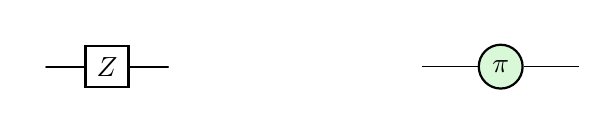
\begin{tikzpicture}
    \node[scale=1.0] (0,0) {
      \begin{quantikz}
        \qw & \gate{Z} & \qw
      \end{quantikz}
    };
    \node [style=gn] (1) at (5,0) {\(\pi\)};
    \draw (4,0) to (1);
    \draw (1) to (6,0);
  \end{tikzpicture}\\
  V ZX-računu to dosežemo s pajkom Z (in \(\alpha=\pi\)). Podobno za X smer.\\
  Vrata C-NOT postanejo\vspace{3mm}\\
  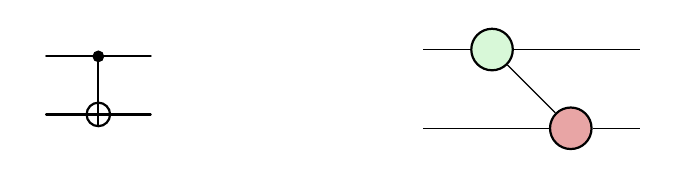
\begin{tikzpicture}
    \node (quantum) at (0,0.5) {
      \begin{quantikz}
        \qw & \ctrl{1} & \qw \\
        \qw & \targ{}  & \qw
      \end{quantikz}
    };
    \node (0) at (4, 0.00) {};
    \node (1) at (4, 1.00) {};
    \node [style=gn] (3) at (5, 1.00) {};
    \node [style=rn] (2) at (6, 0.00) {};
    \node (4) at (7, 0.00) {};
    \node (5) at (7, 1.00) {};
    \draw (0) to (2);
    \draw (1) to (3);
    \draw (2) to (3);
    \draw (2) to (4);
    \draw (3) to (5);
  \end{tikzpicture}\\
  Zgornji kubit pusti nespremenjen, spodnjega negira.
\end{frame}
\begin{frame}
  \frametitle{Pravila}
  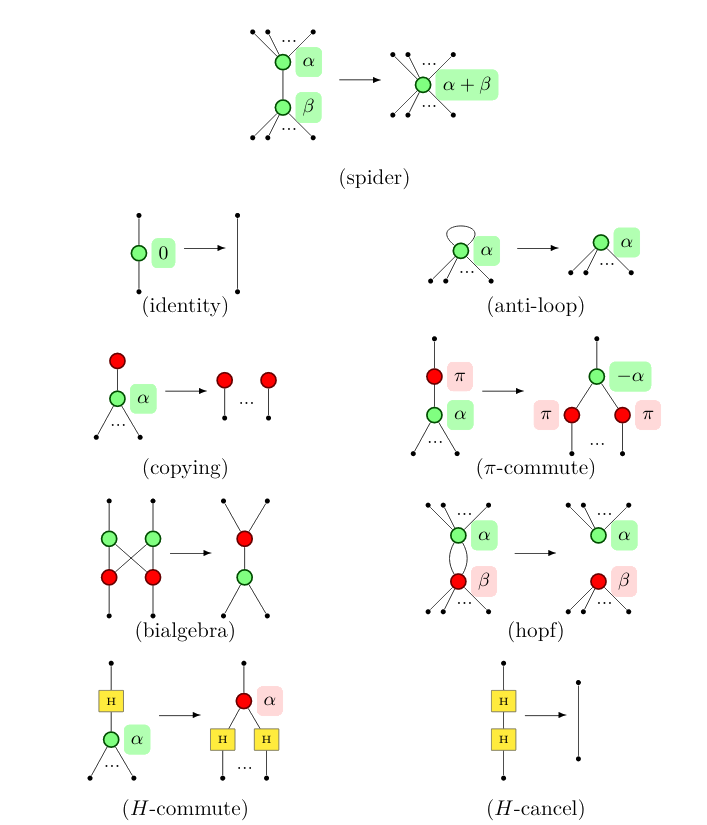
\includegraphics[height=0.9\textheight]{pravila_trans}
\end{frame}
\begin{frame}[fragile]
  \frametitle{Kvantna teleportacija}
  \begin{itemize}
  \item Želimo prenesti kubit na dolge razdalje, ne da bi ga fizično transportirali.
  \item Pomagamo si s parom prepletenih delcev
  \end{itemize}
  Bellova delca A in B\\
  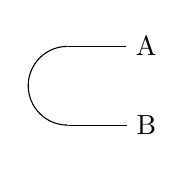
\begin{tikzpicture}
    \node (01) at (1, 0) {A};
    \node (11) at (1, -1) {B};
    \draw (0,0) arc (90:270:0.5);
    \draw (0,0) to (01);
    \draw (0,-1) to (11);
  \end{tikzpicture}\\
  Pred komunikacijo delec A pošljemo na ciljno lokacijo, B pa na začetek
\end{frame}
\begin{frame}
  \frametitle{Kvantna teleportacija}
  Dodamo vhodni kubit\\
  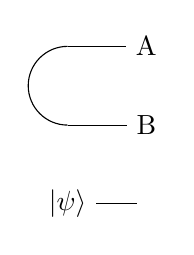
\begin{tikzpicture}
    \node (01) at (1, 0) {A};
    \node (11) at (1, -1) {B};
    \node (input) at (0,-2) {\(\ket\psi\)};
    \node (inconn) at (1,-2) {};
    \draw (0,0) arc (90:270:0.5);
    \draw (0,0) to (01);
    \draw (0,-1) to (11);
    \draw (input) to (inconn);
  \end{tikzpicture}
\end{frame}
\begin{frame}
  \frametitle{Kvantna teleportacija}
  Bellov delec združimo z vhodom.\\
  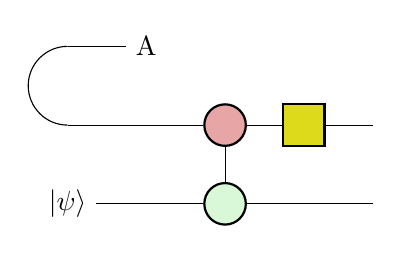
\begin{tikzpicture}
    \node (01) at (1, 0) {A};
    \node (input) at (0,-2) {\(\ket\psi\)};
    \node [style=gn] (bellg) at (2,-2) {};
    \node [style=rn] (bellr) at (2,-1) {};
    \node [style=had] (bellh) at (3,-1) {};
    \node (emptyoutr) at (4, -1) {};
    \node (emptyoutg) at (4, -2) {};
    \draw (0,0) arc (90:270:0.5);
    \draw (0,0) to (01);
    \draw (0,-1) to (bellr);
    \draw (bellr) to (bellh);
    \draw (bellr) to (bellg);
    \draw (input) to (bellg);
    \draw (emptyoutg) to (bellg);
    \draw (emptyoutr) to (bellh);
  \end{tikzpicture}\\
  Ta način združitve ustreza rotaciji Bellove baze na X bazo.
\end{frame}
\begin{frame}
  \frametitle{Kvantna teleportacija}
  Izmerimo možne rezultate združitve.\\
  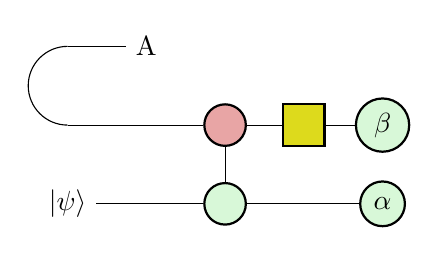
\begin{tikzpicture}
    \node (01) at (1, 0) {A};
    \node (input) at (0,-2) {\(\ket\psi\)};
    \node [style=gn] (bellg) at (2,-2) {};
    \node [style=rn] (bellr) at (2,-1) {};
    \node [style=had] (bellh) at (3,-1) {};
    \node [style=gn] (measurea) at (4,-1) {\(\beta\)};
    \node [style=gn] (measureb) at (4,-2) {\(\alpha\)};
    %
    \draw (0,0) arc (90:270:0.5);
    \draw (0,0) to (01);
    \draw (0,-1) to (bellr);
    \draw (bellr) to (bellh);
    \draw (bellr) to (bellg);
    \draw (input) to (bellg);
    \draw (measureb) to (bellg);
    \draw (measurea) to (bellh);
  \end{tikzpicture}\\
  Kjer \(\alpha, \beta \in \{0,\pi\}\) (ugotovimo jih po meritvi)
\end{frame}
\begin{frame}
  \frametitle{Kvantna teleportacija}
  Pošljemo \(\alpha, \beta\) do druge osebe, ta naredi popravek na svojem kubitu
  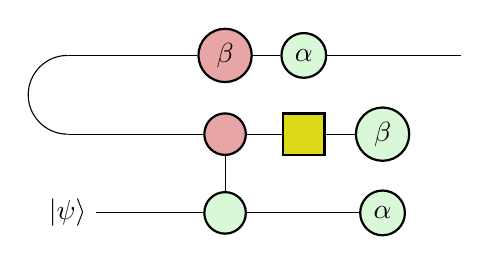
\begin{tikzpicture}
    \node (input) at (0,-2) {\(\ket\psi\)};
    \node [style=gn] (bellg) at (2,-2) {};
    \node [style=rn] (bellr) at (2,-1) {};
    \node [style=had] (bellh) at (3,-1) {};
    \node [style=gn] (measurea) at (4,-1) {\(\beta\)};
    \node [style=gn] (measureb) at (4,-2) {\(\alpha\)};
    \node [style=rn] (correctionr) at (2, 0) {\(\beta\)};
    \node [style=gn] (correctiong) at (3, 0) {\(\alpha\)};
    %
    \draw (0,0) arc (90:270:0.5);
    \draw (0,0) to (correctionr);
    \draw (correctionr) to (correctiong);
    \draw (correctiong) to (5,0);
    \draw (0,-1) to (bellr);
    \draw (bellr) to (bellh);
    \draw (bellr) to (bellg);
    \draw (input) to (bellg);
    \draw (measureb) to (bellg);
    \draw (measurea) to (bellh);
  \end{tikzpicture}
\end{frame}
\begin{frame}
  \frametitle{Kvantna teleportacija}
  Poenostavljanje\\
  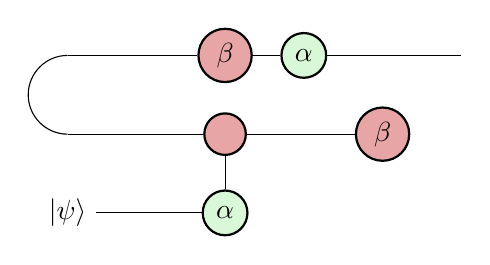
\begin{tikzpicture}
    \node (input) at (0,-2) {\(\ket\psi\)};
    \node [style=gn] (bellg) at (2,-2) {\(\alpha\)};
    \node [style=rn] (bellr) at (2,-1) {};
    \node [style=rn] (measurea) at (4,-1) {\(\beta\)};
    \node [style=rn] (correctionr) at (2, 0) {\(\beta\)};
    \node [style=gn] (correctiong) at (3, 0) {\(\alpha\)};
    %
    \draw (0,0) arc (90:270:0.5);
    \draw (0,0) to (correctionr);
    \draw (correctionr) to (correctiong);
    \draw (correctiong) to (5,0);
    \draw (0,-1) to (bellr);
    \draw (bellr) to (measurea);
    \draw (bellr) to (bellg);
    \draw (input) to (bellg);
  \end{tikzpicture}
\end{frame}
\begin{frame}
  \frametitle{Kvantna teleportacija}
  Poenostavljanje\\
  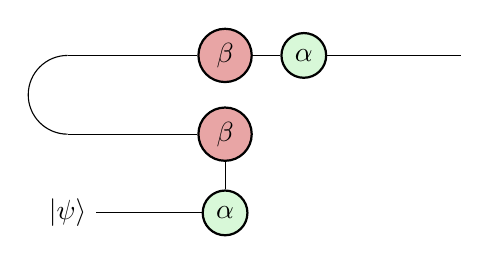
\begin{tikzpicture}
    \node (input) at (0,-2) {\(\ket\psi\)};
    \node [style=gn] (bellg) at (2,-2) {\(\alpha\)};
    \node [style=rn] (bellr) at (2,-1) {\(\beta\)};
    \node [style=rn] (correctionr) at (2, 0) {\(\beta\)};
    \node [style=gn] (correctiong) at (3, 0) {\(\alpha\)};
    %
    \draw (0,0) arc (90:270:0.5);
    \draw (0,0) to (correctionr);
    \draw (correctionr) to (correctiong);
    \draw (correctiong) to (5,0);
    \draw (0,-1) to (bellr);
    \draw (bellr) to (bellg);
    \draw (input) to (bellg);
  \end{tikzpicture}
\end{frame}
\begin{frame}
  \frametitle{Kvantna teleportacija}
  Poenostavljanje\vspace{5mm}\\
  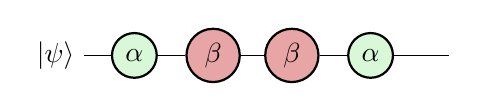
\begin{tikzpicture}
    \node (input) at (0,0) {\(\ket\psi\)};
    \node [style=gn] (bellg) at (1,0) {\(\alpha\)};
    \node [style=rn] (bellr) at (2,0) {\(\beta\)};
    \node [style=rn] (correctionr) at (3, 0) {\(\beta\)};
    \node [style=gn] (correctiong) at (4, 0) {\(\alpha\)};
    %
    \draw (input) to (bellg);
    \draw (bellg) to (bellr);
    \draw (correctionr) to (bellr);
    \draw (correctionr) to (correctiong);
    \draw (correctiong) to (5,0);
  \end{tikzpicture}
\end{frame}
\begin{frame}
  \frametitle{Kvantna teleportacija}
  Poenostavljanje\vspace{5mm}\\
  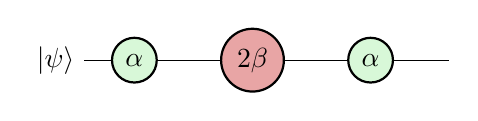
\begin{tikzpicture}
    \node (input) at (0,0) {\(\ket\psi\)};
    \node [style=gn] (bellg) at (1,0) {\(\alpha\)};
    \node [style=rn] (bellr) at (2.5,0) {\(2\beta\)};
    \node [style=gn] (correctiong) at (4, 0) {\(\alpha\)};
    %
    \draw (input) to (bellg);
    \draw (bellg) to (bellr);
    \draw (bellr) to (correctiong);
    \draw (correctiong) to (5,0);
  \end{tikzpicture}
\end{frame}
\begin{frame}
  \frametitle{Kvantna teleportacija}
  Ker je \(\beta \in \{0, \pi\}\) se \(2\beta\) izniči\\
  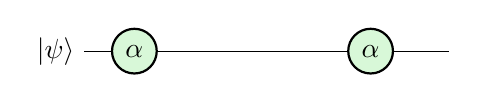
\begin{tikzpicture}
    \node (input) at (0,0) {\(\ket\psi\)};
    \node [style=gn] (bellg) at (1,0) {\(\alpha\)};
    \node [style=gn] (correctiong) at (4, 0) {\(\alpha\)};
    %
    \draw (input) to (bellg);
    \draw (bellg) to (correctiong);
    \draw (correctiong) to (5,0);
  \end{tikzpicture}
\end{frame}
\begin{frame}
  \frametitle{Kvantna teleportacija}
  Dobimo ravno črto, ki je očitno identiteta.\vspace{5mm}\\
  \begin{tikzpicture}
    \node (input) at (0,0) {\(\ket\psi\)};
    \node (output) at (5,0) {\(\ket\psi\)};
    %
    \draw (input) to (output);
  \end{tikzpicture}\\
  \vspace{3mm}Torej smo na izhodu dobili isti kubit kot na vhodu (čeprav ju nismo fizično premikali od ene točke do druge)!
\end{frame}
\end{document}